\documentclass{exam}

\usepackage{units} 
\usepackage{graphicx}
\usepackage[fleqn]{amsmath}
\usepackage{cancel}
\usepackage{float}
\usepackage{mdwlist}
\usepackage{booktabs}
\usepackage{cancel}
\usepackage{polynom}
\usepackage{caption}
\usepackage{fullpage}
\usepackage{comment}
\usepackage{enumerate}
\usepackage{xfrac}
\usepackage{parskip}

\newcommand{\dg}{\ensuremath{^\circ}} 
\everymath{\displaystyle}

\printanswers
\excludecomment{comment}

\ifprintanswers 
  \usepackage{2in1, lscape} 
\fi

\author{}
\date{December 17, 2014}
\title{Math 142 \\ Homework Thirteen}

\begin{document}

  \maketitle

  \section{Homework}
  Section 7.2: 1-4, 9-17, 23-27, 30-38, 41-44

  \section{Extra Credit}
  Section 7.2: 48 and 49

  \ifprintanswers
    \pagebreak
    \begin{enumerate}

      \item[87] 
        \begin{align*}
          (\tan x + \cot x)^4 & = \left[ (\tan x + \cot x)^2 \right]^2 \\
                              & = \left( \tan^2 x + 2 \tan x \cot x + \cot^2 x \right)^2 \\
                              & = \left( \tan^2 x + 2 + \cot^2 x \right)^2 \\
                              & = \left( \sec^2 x - 1 + 2 + \csc^2 x - 1 \right)^2 \\
                              & = \left( \sec^2 x + \csc^2 x \right)^2 \\
                              & = \left( \frac{1}{\cos^2 x} + \frac{1}{\sin^2 x} \right)^2 \\
                              & = \left( \frac{\sin^2 x + \cos^2 x}{\sin^2 x \cos^2 x} \right)^2 \\
                              & = \left( \frac{1}{\sin^2 x \cos^2 x} \right)^2 \\
                              & = \csc^4 x \sec^4 x \\
        \end{align*}

    \end{enumerate}
  \fi

  \section{Review}

  \ifprintanswers
    \section{Section 7.1}
    \begin{description}

      \item[1] 
        \begin{align*}
          \sin 75 \dg & = \sin (45 \dg + 30 \dg) \\
                      % & = \sin 45 \dg \cos 30 \dg + \cos 45 \dg \sin 30 \dg \\
                      % & = \frac{\sqrt{2}}{2} \cdot \frac{\sqrt{3}}{2} + \frac{\sqrt{2}}{2} \cdot \frac{1}{2} \\
                      & = \boxed{ \frac{\sqrt{6} + \sqrt{2}}{4} } \\
        \end{align*}

      \item[2] 
        \begin{align*}
          \sin 15 \dg & = \sin (45 \dg - 30 \dg) \\
                      % & = \sin 45 \dg \cos 30 \dg - \cos 45 \dg \sin 30 \dg \\
                      % & = \frac{\sqrt{2}}{2} \cdot \frac{\sqrt{3}}{2} - \frac{\sqrt{2}}{2} \cdot \frac{1}{2} \\
                      & = \boxed{ \frac{\sqrt{6} - \sqrt{2}}{4} } \\
        \end{align*}

      \item[3] 
        \begin{align*}
          \cos 105 \dg & = \cos (45 \dg + 60 \dg) \\
                      % & = \cos 45 \dg \cos 60 \dg - \sin 45 \dg \sin 60 \dg \\
                      % & = \frac{\sqrt{2}}{2} \cdot \frac{1}{2} - \frac{\sqrt{2}}{2} \cdot \frac{\sqrt{3}}{2} \\
                      & = \boxed{ \frac{\sqrt{2} - \sqrt{6}}{4} } \\
        \end{align*}

      \item[4] 
        \begin{align*}
          \cos 195 \dg & = \cos (135 \dg + 60 \dg) \\
                      % & = \cos 135 \dg \cos 60 \dg - \sin 135 \dg \sin 60 \dg \\
                      % & = - \frac{\sqrt{2}}{2} \cdot \frac{1}{2} - \frac{\sqrt{2}}{2} \cdot \frac{\sqrt{3}}{2} \\
                      & = \boxed{ \frac{- \sqrt{2} - \sqrt{6}}{4} } \\
        \end{align*}

      \item[9] 
        \begin{align*}
          \tan \left( - \sfrac{\pi}{12} \right) &= \tan \left( \sfrac{\pi}{6} - \sfrac{\pi}{3} \right) \\
          % &= \frac{\tan \sfrac{\pi}{6} - \tan \sfrac{\pi}{3}}{1 + \tan \sfrac{\pi}{6} \tan \sfrac{\pi}{3}} \\
          &= \boxed{ \sqrt{3} - 2 } \\
        \end{align*}

      \item[10] 
        \begin{align*}
          \sin \left( - \sfrac{5 \pi}{12} \right) & = - \sin \left( \sfrac{5 \pi}{12} \right) \\
                                                  & = - \sin \left( \sfrac{\pi}{4} + \sfrac{\pi}{6} \right) \\
                                                  & = \boxed{ \frac{- \sqrt{2} - \sqrt{6}}{4} } \\
        \end{align*}

      \item[11] 
        \begin{align*}
          \cos \left( \sfrac{11 \pi}{12} \right) & = \cos \left( \sfrac{3 \pi}{12} + \sfrac{8 \pi}{12} \right) \\
                                                 & = \cos \left( \sfrac{\pi}{4} + \sfrac{2 \pi}{3} \right) \\
                                                 & = \boxed{ \frac{- \sqrt{2} - \sqrt{6}}{4} } \\
        \end{align*}

      \item[12] 
        \begin{align*}
          \cos \left( \sfrac{7 \pi}{12} \right) & = \cos \left( \sfrac{3 \pi}{12} + \sfrac{4 \pi}{12} \right) \\
                                                & = \cos \left( \sfrac{\pi}{4} + \sfrac{\pi}{3} \right) \\
                                                & = \boxed{ \frac{\sqrt{2} - \sqrt{6}}{4} } \\
        \end{align*}

      \item[13] 
        \begin{align*}
          \sin 18 \dg \cos 27 \dg + \cos 18 \dg \sin 27 \dg & = \sin (18 \dg + 27 \dg) \\
                                                            & = \sin 45 \dg \\
                                                            & = \boxed{ \frac{\sqrt{2}}{2} } \\
        \end{align*}

      \item[14] 
        \begin{align*}
          \cos 10 \dg \cos 80 \dg - \sin 10 \dg \sin 80 \dg & = \cos (10 \dg + 80 \dg) \\
                                                            & = \cos 90 \dg \\
                                                            & = \boxed{ 0 } \\
        \end{align*}

      \item[15] 
        \begin{align*}
          \cos \frac{3 \pi}{7}  \cos \frac{2 \pi}{21}  + \sin \frac{3 \pi}{7}  \sin \frac{2 \pi}{21} 
            & = \cos \left( \frac{3 \pi}{7}  - \frac{2 \pi}{21} \right) \\
            & = \cos \frac{\pi}{3} \\
            & = \boxed{ \frac{1}{2} } \\
        \end{align*}

      \item[16] 
        \begin{align*}
          \frac{\tan \frac{\pi}{18} + \tan \frac{\pi}{9}}{1 - \tan \frac{\pi}{18} \tan \frac{\pi}{9}} 
            &= \tan \left( \frac{\pi}{18} + \frac{\pi}{9} \right) \\
            &= \tan \frac{\pi}{3} \\
            &= \boxed{ \sqrt{3} } \\
        \end{align*}

      \item[17] 
        \begin{align*}
          \sin \left( \frac{\pi}{2} - u \right) & = \sin \frac{\pi}{2} \cos u - \cos \frac{\pi}{2} \sin u \\
                                                & = \cos u \\
          \\
          \cos \left( \frac{\pi}{2} - u \right) & = \cos \frac{\pi}{2} \cos u + \sin \frac{\pi}{2} \sin u \\
                                                & = \sin u \\
          \\
          \tan \left( \frac{\pi}{2} - u \right) 
            & = \frac{\sin \left( \sfrac{\pi}{2} - u \right)}{\cos \left( \sfrac{\pi}{2} - u \right)} \\
            & = \frac{\cos u}{\sin u} \\
            & = \cot u \\
        \end{align*}

      \item[23] 
        \begin{align*}
          \sin \left( x - \frac{\pi}{2} \right) & = \sin x \cos \frac{\pi}{2} - \cos x \sin \frac{\pi}{2} \\
                                                & = - \cos x \\
        \end{align*}

      \item[24] 
        \begin{align*}
          \cos \left( x - \frac{\pi}{2} \right) & = \cos x \cos \frac{\pi}{2} + \sin x \sin \frac{\pi}{2} \\
                                                & = \sin x \\
        \end{align*}

      \item[25] 
        \begin{align*}
          \sin(x - \pi) & = \sin x \cos \pi - \cos x \sin \pi \\
                        & = - \sin x \\
        \end{align*}

      \item[26] 
        \begin{align*}
          \cos(x - \pi) & = \cos x \cos \pi + \sin x \sin \pi \\
                        & = - \cos x \\
        \end{align*}

      \item[27] 
        \begin{align*}
          \tan(x - \pi) & = \frac{\tan x + \tan \pi}{1 - \tan x \tan \pi} \\
                        & = \tan x \\
        \end{align*}

      \item[30] 
        \begin{align*}
          \tan \left(x - \frac{\pi}{4} \right) & = \frac{\tan x - \tan \sfrac{\pi}{4}}{1 + \tan x \tan \sfrac{\pi}{4}} \\
                                               & = \frac{\tan x - 1}{\tan x + 1} \\
        \end{align*}

      \item[31] 
        \begin{align*}
          \sin(x + y) & - \sin(x - y) \\
                      & = (\sin x \cos y + \cos x \sin y) - (\sin x \cos y - \cos x \sin y) \\
                      & = \sin x \cos y + \cos x \sin y - \sin x \cos y + \cos x \sin y \\
                      & = 2 \cos x \sin y \\
        \end{align*}

      \item[32] 
        \begin{align*}
          \cos(x + y) & + \cos(x - y) \\
                      & = (\cos x \cos y - \sin x \sin y) + (\cos x \cos y + \sin x \sin y) \\
                      & = \cos x \cos y - \sin x \sin y + \cos x \cos y + \sin x \sin y \\
                      & = 2 \cos x \cos y \\
        \end{align*}

      \item[33] 
        \begin{align*}
          \cot(x - y) & = \frac{1}{\tan(x - y)} \\
                      & = \frac{1 + \tan x \tan y}{\tan x - \tan y} \cdot \frac{\sfrac{1}{\tan x \tan y}}{\sfrac{1}{\tan x \tan y}} \\
                      & = \frac{\cot x \cot y + 1}{\cot y - \cot x} \\
        \end{align*}

      \item[34] 
        \begin{align*}
          \cot(x + y) & = \frac{1}{\tan(x + y)} \\
                      & = \frac{1 - \tan x \tan y}{\tan x + \tan y} \cdot \frac{\sfrac{1}{\tan x \tan y}}{\sfrac{1}{\tan x \tan y}} \\
                      & = \frac{\cot x \cot y - 1}{\cot x + \cot y} \\
        \end{align*}

      \item[35] 
        \begin{align*}
          \frac{\sin(x - y)}{\cos x \cos y} & = \frac{\sin x \cos y - \cos x \sin y}{\cos x \cos y} \\
                                            & = \tan x - \tan y \\
        \end{align*}

      \item[36] 
        \begin{align*}
          \frac{\cos(x + y)}{\cos x \cos y} & = \frac{\cos x \cos y - \sin x \sin y}{\cos x \cos y} \\
                                            & = 1 - \tan x \tan y \\
        \end{align*}

      \item[37] 
        \begin{align*}
          & \frac{\sin(x + y) - \sin(x - y)}{\cos(x + y) + \cos(x - y)} \\
          & = \frac{(\sin x \cos y + \cos x \sin y) - (\sin x \cos y - \cos x \sin y)}{(\cos x \cos y - \sin x \sin y) + (\cos x \cos y + \sin x \sin y)} \\
          & = \frac{\sin x \cos y + \cos x \sin y - \sin x \cos y + \cos x \sin y}{\cos x \cos y - \sin x \sin y + \cos x \cos y + \sin x \sin y} \\
          & = \frac{2 \cos x \sin y}{2 \cos x \cos y} \\
          & = \tan y \\
        \end{align*}

      \item[38] 
        \begin{align*}
          \cos(x + y) \cos(x - y) & = ( \cos x \cos y - \sin x \sin y )( \cos x \cos y + \sin x \sin y ) \\
                                  & = \cos^2 x \cos^2 y - \sin^2 x \sin^2 y \\
                                  & = \cos^2 x \left( 1 - \sin^2 y \right) - \sin^2 x \sin^2 y \\
                                  & = \cos^2 x - \cos^2 x \sin^2 y  - \sin^2 x \sin^2 y \\
                                  & = \cos^2 x - \sin^2 y \left( \cos^2 x + \sin^2 x \right) \\
                                  & = \cos^2 x - \sin^2 y \\
        \end{align*}

      \item[41] 
        find k:
        \begin{align*}
          k & = \sqrt{(-3)^2 + 1^2} \\
            & = 2 \\
        \end{align*}

        Since $\cos \phi < 0$ and $\sin \phi > 0$, $\phi$ is in Q-II:
        \begin{align*}
          \cos \phi & = - \frac{\sqrt{3}}{2} \\
          \sin \phi & = \frac{1}{2} \\
          \phi      & = \frac{5 \pi}{6} \\
        \end{align*}

        The equation is:
        \[
          - \sqrt{3} \sin x + \cos x = \boxed{ 2 \sin \left( x + \frac{5 \pi}{6} \right) } 
        \]

        \begin{figure}[H]
          \centering
          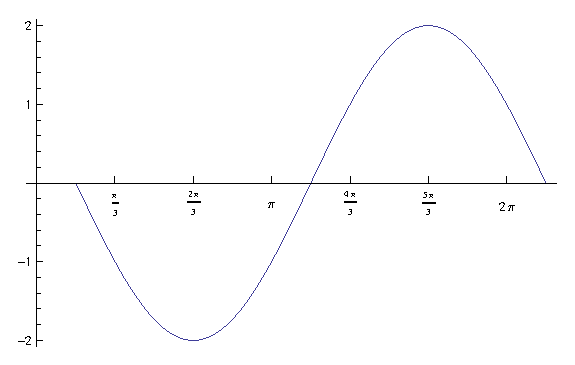
\includegraphics[scale=0.8]{problem41.eps}
          \caption{Problem 41}
        \end{figure}

      \item[42] 
        find k:
        \begin{align*}
          k & = \sqrt{1^2 + 1^2} \\
            & = \sqrt{2} \\
        \end{align*}

        Since $\cos \phi > 0$ and $\sin \phi > 0$, $\phi$ is in Q-I:
        \begin{align*}
          \cos \phi & = \frac{\sqrt{2}}{2} \\
          \sin \phi & = \frac{\sqrt{2}}{2} \\
          \phi      & = \frac{\pi}{4} \\
        \end{align*}

        The equation is:
        \[
          \sin x + \cos x = \boxed{ \sqrt{2} \sin \left( x + \frac{\pi}{4} \right) } 
        \]

        \begin{figure}[H]
          \centering
          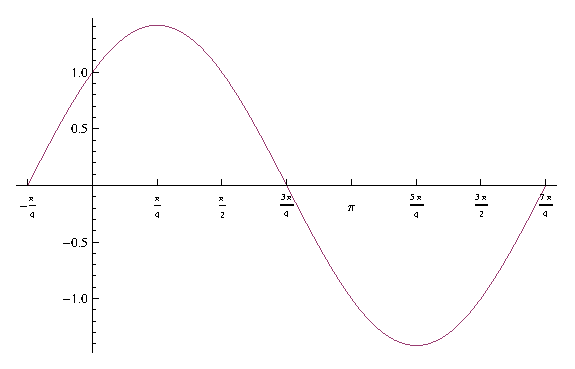
\includegraphics[scale=0.8]{problem42.eps}
          \caption{Problem 42}
        \end{figure}

      \item[43] 
        find k:
        \begin{align*}
          k & = \sqrt{5^2 + 5^2} \\
            & = 5 \sqrt{2} \\
        \end{align*}

        Since $\cos \phi > 0$ and $\sin \phi < 0$, $\phi$ is in Q-IV:
        \begin{align*}
          \cos \phi & = \frac{\sqrt{2}}{2} \\
          \sin \phi & = - \frac{\sqrt{2}}{2} \\
          \phi      & = \frac{7 \pi}{4} \\
        \end{align*}

        The equation is:
        \[
          5 \sin 2x - 5 \cos 2x = \boxed{ 5 \sqrt{2} \sin \left( 2x + \frac{7 \pi}{4} \right) } 
        \]

        \begin{figure}[H]
          \centering
          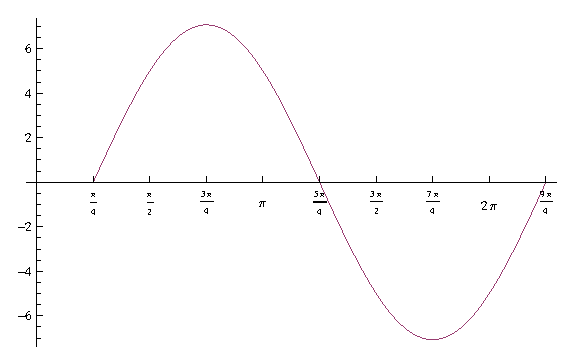
\includegraphics[scale=0.8]{problem43.eps}
          \caption{Problem 43}
        \end{figure}

      \item[44] 
        find k:
        \begin{align*}
          k & = \sqrt{3^2 + (3 \sqrt{3})^2} \\
            & = 6 \\
        \end{align*}

        Since $\cos \phi > 0$ and $\sin \phi > 0$, $\phi$ is in Q-I:
        \begin{align*}
          \cos \phi & = \frac{1}{2} \\
          \sin \phi & = \frac{\sqrt{3}}{2} \\
          \phi      & = \frac{\pi}{3} \\
        \end{align*}

        The equation is:
        \[
          3 \sin \pi x + 3 \sqrt{3} \cos \pi x = \boxed{6 \sin \left( x + \frac{\pi}{3} \right)} 
        \]

        \begin{figure}[H]
          \centering
          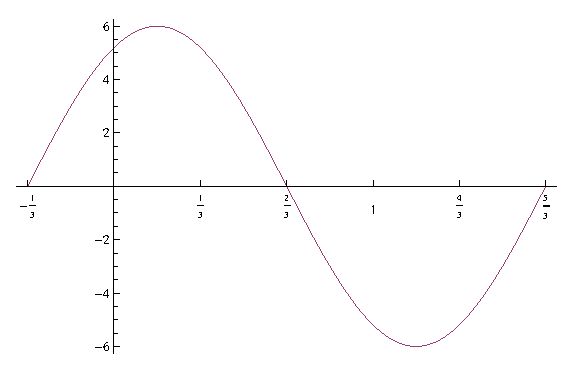
\includegraphics[scale=0.8]{problem44.eps}
          \caption{Problem 44}
        \end{figure}

    \end{description}

  \else
    \vspace{5 cm}

    \begin{quote}
      \begin{em}
      \end{em}
    \end{quote}
    \hspace{1 cm} --TO DO
  \fi

\end{document}

